\documentclass[a4paper]{article}


\usepackage[T1]{fontenc}    
\usepackage[utf8]{inputenc} 
\usepackage{textcomp}      
\date{} 					
\author{}                   
\usepackage{geometry}		
\geometry{ left=2cm, right=2cm, top=2cm, bottom=4cm, bindingoffset=5mm}

\usepackage{graphicx}
\usepackage{xcolor}
\usepackage{hyperref} 
\usepackage{fancyhdr}
\usepackage{amsmath}											
\pagestyle{fancy}
\fancyhf{}
\fancyhead[R]{2973140 - Felix Bühler  \\ 2893121 - Jan Leusmann \\  3141241 - Jamie Ullerich}
\fancyhead[L]{Scientific Visualisation \\ Sommersemester 2019 }
\renewcommand{\headrulewidth}{0.5pt} 				

\title{Exercise 6}

\begin{document}

\maketitle 
\thispagestyle{fancy}


\section*{Exercise 6.1}

Figure \ref{fig:triangle} shows a rectangle which consists of two adjacent triangles and a point p. 
When interpolating this point inside the rectangle, all corners (1 - 4) are considered. 
But, the colour of point p will be different when interpolating inside the left triangle only the corners 1, 2 and 3 will be considered. 
There is an even higher difference when point p is near the centre of the rectangle. 
This effect increases when the triangle has a acute angle, because then the corners ca be far away and therefore the colour will be different. 
Having a triangulation that satisfies the Delaunay properties may decrease this effect. 
So in general the triangles are distributed more evenly and the difference of colour is less. 

\begin{figure}[h!]
	\centering 
	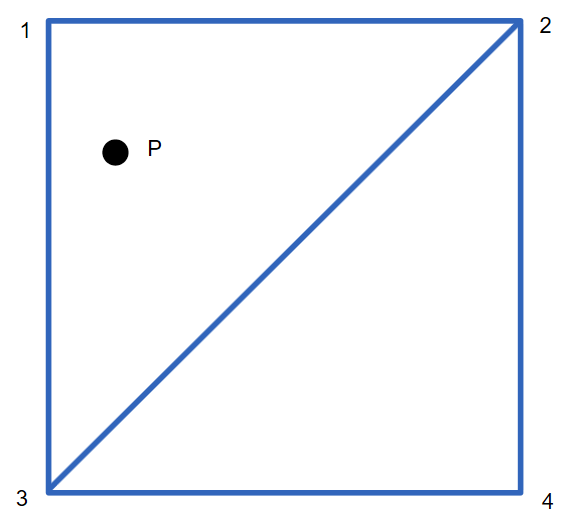
\includegraphics[width=5cm]{A1.png}
	\caption{}
	\label{fig:triangle}
\end{figure}

\section*{Exercise 6.2}


\section*{Exercise 6.3}

\subsection*{6.3.1}
Nyquist - Shannon Theorem:
The minimum sampling frequency of a signal that it will not distort its underlying information, should be double the frequency of its highest frequency component.\\
$ \nu_s \leq \dfrac{1}{2} * \nu_x $

\newpage
\subsection*{6.3.2}
\begin{figure}[!ht]
	\centering
	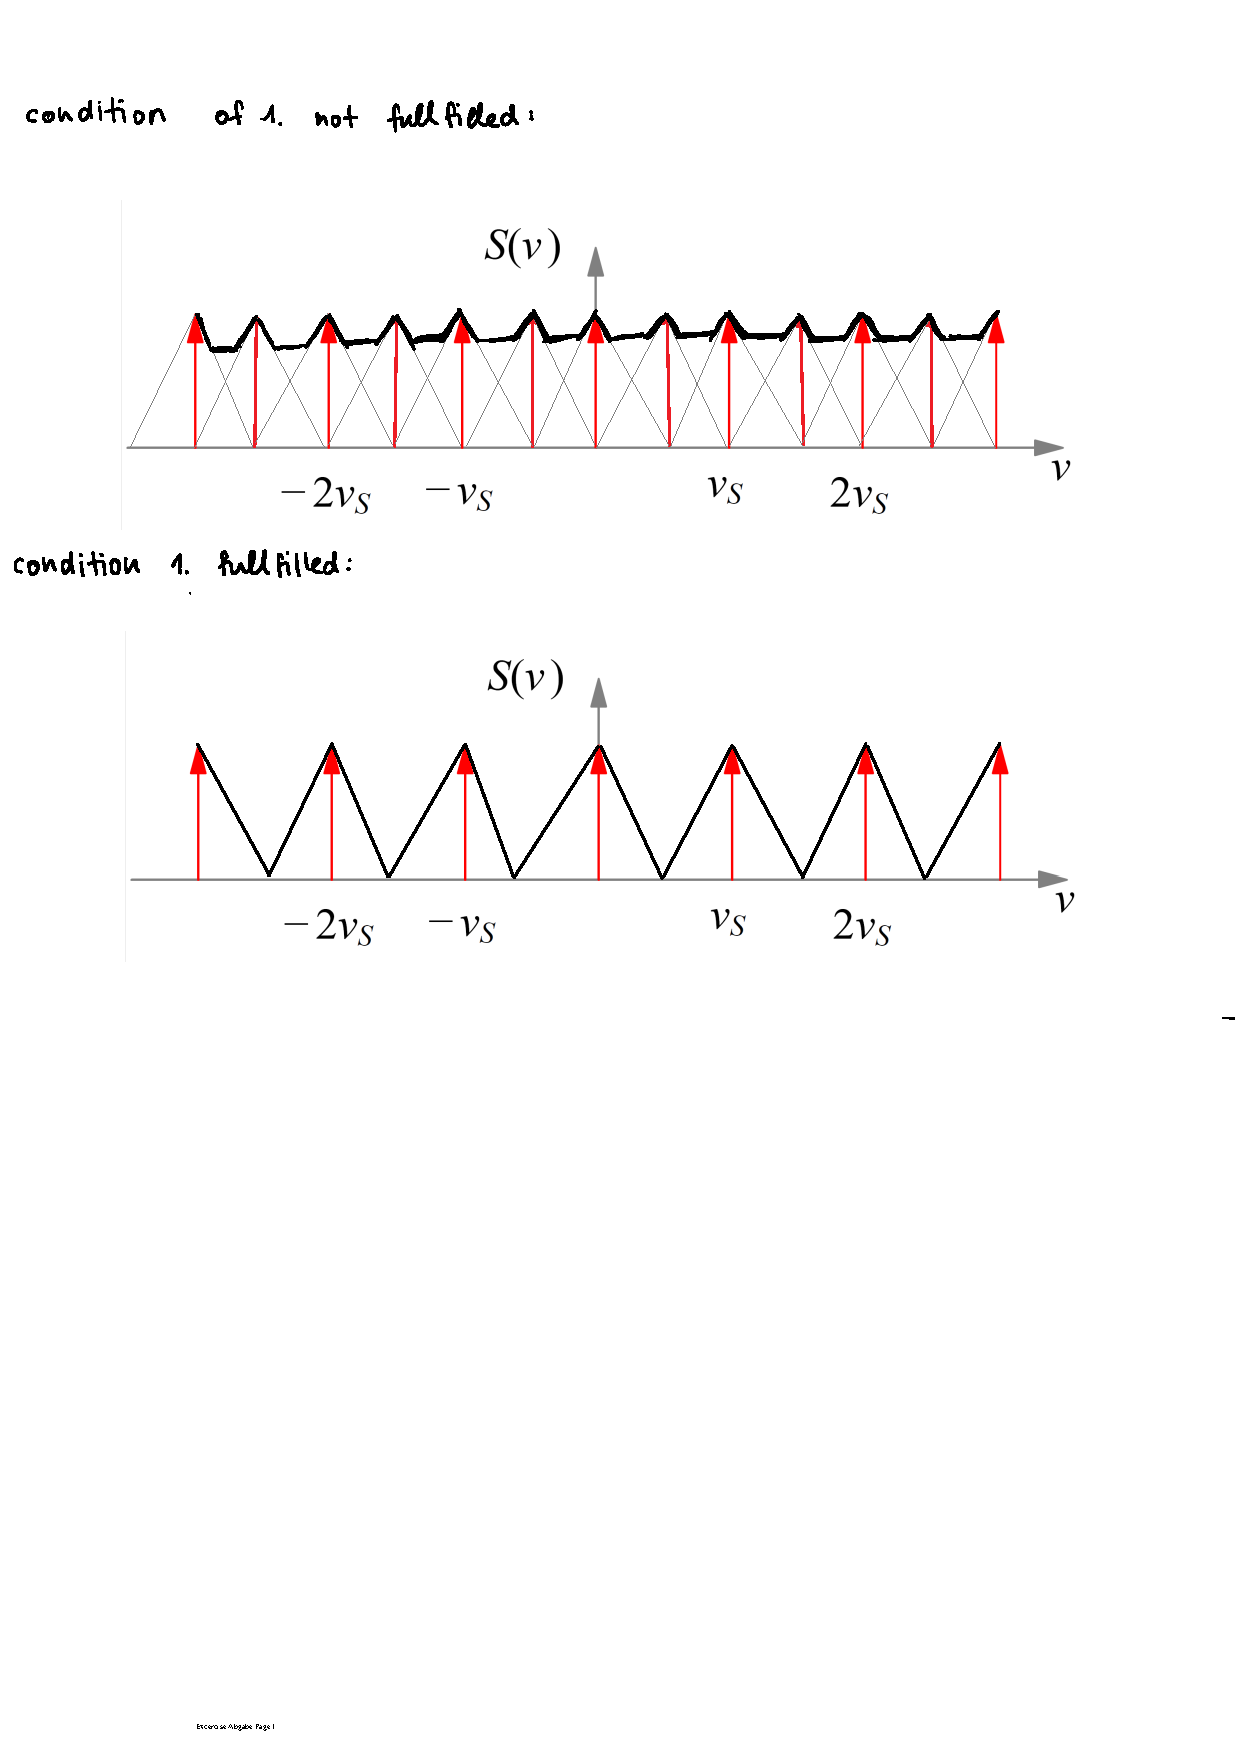
\includegraphics[width=0.79\linewidth]{6_3_2.pdf}
	%\caption{}
	\label{fig:delaunay}
\end{figure}

\subsection*{6.3.3}

\end{document}